\chapter{Background}\label{background}
This chapter provides an overview of various examples of proof systems, the \lstinline{parjs} parsing library, and a comparison of existing educational proof assistants. \Cref{background:proof-systems} presents three proof systems: Natural Deduction, the simply typed $\lambda$-calculus, and the Sequent Calculus \textsc{lk}. They are chosen because the algorithms presented in \Cref{chapter:input} and \Cref{chapter:checking} are primarily tested on variations of these three systems. \Cref{background:parsing} explains why the \lstinline{parjs} library is chosen for the parsing tasks in this project and presents features of \lstinline{parjs} that guide certain algorithm design decisions. Finally, \Cref{background:comparison} evaluates numerous logic learning tools based on user experience and flexibility to support numerous proof systems, then summarises common features that guide the development of the application.

\section{Proof systems}
\label{background:proof-systems}
This section presents an overview of Natural Deduction \ndt{}, the simply typed $\lambda$-calculus, and the Sequent Calculus \textsc{lk}. They are pre-defined in the web application, and on which most of the algorithm development is based.

\subsection{Natural Deduction \texorpdfstring{\ndt{}}{with implication}}
In 1934, Gerhard Gentzen introduced the Natural Deduction systems \textsc{nj} and \textsc{nk} \cite{gentzen:1969}. This section gives the definition of \ndt{}, a subsystem of Natural Deduction which has implication ($\to$) as the only logical connective.
\begin{definition}[Formulae in \ndt{}]
    The formulae in $\textsc{nd}_\to$ are:
    \[
        A, B \Coloneqq x \alt (A \to B)
    \]
    where $x$ can be any symbol from an infinite list $a, b, c, \ldots, x, y, z \ldots$ of term variables.
\end{definition}
\begin{definition}[Contexts in \ndt{}]
    A \textit{context} $\Gamma$ is an unordered multiset of formulae. The notation $\Gamma, A$ is equivalent to the multiset union $\Gamma \cup \{ A \}$, which adds the term $A$ to $\Gamma$ regardless of whether $A$ appears in $\Gamma$.
\end{definition}
\begin{definition}[Judgements in \ndt{}]
    A \textit{judgement} (or \textit{statement}) takes the form $\Gamma \vdash A$. It means ``if all the formulae in $\Gamma$ hold, then $A$ holds''.
\end{definition}
\begin{definition}[Inference rules in \ndt{}]
    The inference rules are defined as follows:
    {
        \derivationfont
        \[
            (Ax): \frac{}{\Gamma, A \vdash A} \tquad (\arr I): \frac{\Gamma, A \vdash B}{\Gamma \vdash (A \to B)} \tquad (\arr E): \frac{\Gamma \vdash (A \to B) \quad \Gamma \vdash A}{\Gamma \vdash B}
        \]
    }%
\end{definition}
Of course, it is possible to extend the system with additional logical connectives. Each connective is associated with introduction rules ($\cdot I$), which describe how to construct a proof of the connective, and elimination rules ($\cdot E$), which describe how to use a connective. An introduction rule adds the connective to the right of the turnstile, while an elimination rule removes the connective from the right of the turnstile.

For example, the system \ndt{} above can easily be extended with the conjunction operator ($\land$):
{
    \derivationfont
    \[
        (\land I): \frac{\Gamma \vdash A \quad \Gamma \vdash B}{\Gamma \vdash (A \land B)} \tquad (\land E_L): \frac{\Gamma \vdash (A \land B)}{\Gamma \vdash A} \tquad (\land E_R): \frac{\Gamma \vdash (A \land B)}{\Gamma \vdash B}
    \]
}%

\subsubsection{Choice of notation}
In Gentzen's original formulation \cite{gentzen:1969}, there are neither contexts nor turnstiles. Each statement only consists of a formula. The $(\arr I)$ rule in the original formulation can refer to any term arbitrarily higher up in the derivation. It is not \textit{localised}, since it does not always only depend on the premises and conclusion immediately above and below the dividing line. On the contrary, the formulation presented above is \textit{localised}, since all rules only depend on the premises and conclusion immediately above and below the dividing line. The differences between Gentzen's original formulation and the formulation above are highlighted in \Cref{fig:background:natural-deduction}.

\begin{figure}[!htbp]
    \centering
    \begin{subfigure}{.48\textwidth}
        \centering
        \[
            \Inf[\textcolor{ForestGreen}{\arr I^u}]
                {\Inf[\textcolor{blue}{\arr I^v}]
                     {\textcolor{blue}{[x]^v}
                      \quad \Inf[\land E]
                                {\textcolor{ForestGreen}{[x \land y]^u}
                                }{y}
                     }{\textcolor{blue}{x \to y}}
                }{\textcolor{ForestGreen}{(x \land y) \to (x \to y)}}
        \]
        \caption{Gentzen's original formulation}
    \end{subfigure}%
    \quad
    \begin{subfigure}{.48\textwidth}
        \centering
        \[
            \Inf[\arr I]
                {\Inf[\arr I]
                     {\Inf[\land E_R]
                          {\Inf[Ax]{x \land y, x \vdash x \land y}
                          }{x \land y, x \vdash y}
                     }{x \land y \vdash x \to y}
                }{\varnothing \vdash (x \land y) \to (x \to y)}
        \]
        \caption{Localised formulation}
    \end{subfigure}
    \caption{An example derivation highlighting the differences between Gentzen's original formulation of Natural Deduction and a localised formulation}
    \label{fig:background:natural-deduction}
\end{figure}

This project only considers \textit{localised} inference rules, since they are simpler to deal with and are applicable to a wider range of proof systems.

\subsection{Simply typed \lc{}}
In the 1930s, Alonzo Church introduced the (untyped) $\lambda$-calculus \cite{church:1936} as a model of computation that is Turing-complete \cite{turing:1937}. It is the basis of functional programming languages like Haskell, \textsc{ml}, and Lisp.

Church later formulated the simply typed $\lambda$-calculus \cite{church:1940}, which has only one type constructor, $A \to B$, representing function types. This section focuses on type assignment in the manner of Haskell Curry \cite{curry:1934}. In Curry-style type assignment (i.e. \textit{implicit} or \textit{extrinsic} typing), types are assigned to entire $\lambda$-terms. In Church-style type assignment (i.e. \textit{explicit} or \textit{intrinsic} typing) as presented in \cite{church:1940}, types are embedded as variable annotations.

\subsubsection{Why types?}
Types can guarantee the absence of certain errors. For example, the code snippet \lstinline{4.0 / "three"} will not compile in most statically-typed programming languages because \lstinline{"three"} is not a number. However, types can also reject programs that are well-behaved at run-time. For example, a conservative type system may reject the code snippet \lstinline{if true then 10 else "ten"} because \lstinline{10} and \lstinline{"ten"} have different types.

Type annotations can make code more readable. They help clarify the intended usage of variables and functions by supplementing information that are missing from names.

Types can enable certain compiler optimisations, such as using specialised machine instructions for arithmetic operations and determining whether a variable can be allocated on the stack. They allow the compiler to produce more efficient machine code.
\begin{definition}[$\lambda$-terms]
    \label{lambda:lambda-terms}
    $\lambda$-terms are defined as follows \cite{church:1941}:
    \[
        M,N \Coloneqq x \alt \underbracket[0.6pt]{(\lambda x. M)}_\text{abstraction} \alt \underbracket[0.6pt]{(MN)}_\text{application}
    \]
    where $x$ can be any symbol from an infinite list $a, b, c, \ldots, x, y, z \ldots$ of term variables.
\end{definition}
\begin{definition}[Curry types]
    \label{lambda:curry-types}
    \textit{Curry types} (or \textit{simple types}) are defined as follows \cite{van-bakel:2022}:
    \[
        A, B \Coloneqq \varphi \alt (A \rightarrow B)
    \]
    where $\varphi$ can be any symbol from an infinite list $\varphi_1, \varphi_2, \ldots$ of type variables. When writing type variables by hand, it is often more convenient to use the subscript alone to represent a type variable, e.g. the type $((1 \rightarrow 2) \rightarrow 1)$ represents the type $((\varphi_1 \rightarrow \varphi_2) \rightarrow \varphi_1)$. We will only use numbers from this point onwards.
\end{definition}
\begin{definition}[Contexts in Curry type assignment]
    A \textit{context} $\Gamma$ is a set containing elements in the form $x:A$, where $x$ is a variable and $A$ is a Curry type. All variables are assigned at most one type in any context. For example, $x:1, x:2$ is not a well-formed context since $x$ appears twice.
\end{definition}
\begin{definition}[Judgements in Curry type assignment]
    A \textit{judgement} (or \textit{statement}) takes the form $\Gamma \vdash M: A$. It means ``given the type assignments to variables specified by $\Gamma$, the $\lambda$-term $M$ has type $A$''.
\end{definition}
\begin{definition}[Curry type assignment rules]
    \label{lambda:type-assignment}
    $\lambda$-terms can be assigned types under the Curry type assignment system using the following derivation rules \cite{van-bakel:2022}:
    {
        \derivationfont
        \[
            (Ax): \frac{}{\Gamma, x:A \vdash x:A} \quad (\arr I): \frac{\Gamma, x:A \vdash M:B}{\Gamma \vdash (\lambda x. M): (A \to B)} \quad (\arr E): \frac{\Gamma \vdash M: (A \to B) \quad \Gamma \vdash N: A}{\Gamma \vdash (MN): (A \to B)}
        \]
    }%
\end{definition}

\subsection{Sequent Calculus \textsc{lk}}
At the same time as Natural Deduction, Gentzen also introduced the Sequent Calculus \textsc{lk} (standing for \textit{Logistische Kalkül}) \cite{gentzen:1969}, used to build proofs for classical first-order logic. This section considers the system \textsc{lk} restricted to propositional logic.

\begin{definition}[Propositional formulae]
    The subset of propositional formulae relevant to this section are defined as follows:
    \[
        A, B \Coloneqq x \alt (A \to B) \alt (A \land B) \alt (A \lor B) \alt (\lnot A)
    \]
    where $x$ can be any symbol from an infinite list of term variables $a, b, c, \ldots, x, y, z \ldots$ as before.
\end{definition}
\begin{definition}[Judgements in \textsc{lk}]
Each \textit{judgement} (or \textit{statement}, \textit{sequent}) takes the form
\[
    \Gamma \vdash \Delta
\]
where $\Gamma$ and $\Delta$ represent possibly empty, unordered \textit{multiset}s of propositional formulae. Note that $\Gamma$ in the simply typed $\lambda$-calculus is a \textit{set} (i.e. it cannot contain duplicates), while the $\Gamma$ and $\Delta$ here in the system \textsc{lk} are a \textit{multisets} (i.e. they can contain duplicates). When expanded, a statement in the system \textsc{lk} looks like this:
\begin{equation}
    \label{eqn:background:sequent}
    A_1, \ldots, A_n \vdash B_1, \ldots B_m
\end{equation}
where $n, m \geq 0$. It means ``if every $A_1, \ldots, A_n$ is true, then at least one of $B_1, \ldots, B_m$ is true''. Alternatively, the judgement \ref{eqn:background:sequent} holds if and only if
\[
    (A_1 \land \cdots \land A_n) \vdash (B_1 \lor \cdots \lor B_m)
\]
holds.
\end{definition}
\begin{definition}[Inference rules in \textsc{lk}]
    The inference rules are presented as follows:
    \vspace{-11pt}
    \begin{center}
        \derivationfont
        \begin{minipage}{.4\textwidth}
            \begin{align*}
                (Ax) &: \frac{}{A \vdash A} \\[1em]
                (\land L_1) &: \frac{\Gamma, A \vdash \Delta}{\Gamma, (A \land B) \vdash \Delta} \\[1em]
                (\land L_2) &: \frac{\Gamma, B \vdash \Delta}{\Gamma, (A \land B) \vdash \Delta} \\[1em]
                (\lor L) &: \frac{\Gamma, A \vdash \Delta \quad \Gamma, B \vdash \Delta}{\Gamma, (A \lor B) \vdash \Delta} \\[1em]
                (\arr L) &: \frac{\Gamma \vdash A, \Delta \quad \Sigma, B \vdash \Pi}{\Gamma, \Sigma, (A \to B) \vdash \Delta, \Pi} \\[1em]
                (\lnot L) &: \frac{\Gamma \vdash A, \Delta}{\Gamma, (\lnot A) \vdash \Delta} \\[1em]
                (WL) &: \frac{\Gamma \vdash \Delta}{\Gamma, A \vdash \Delta} \\[1em]
                (CL) &: \frac{\Gamma, A, A \vdash \Delta}{\Gamma, A \vdash \Delta}
            \end{align*}
        \end{minipage}%
        \begin{minipage}{.4\textwidth}
            \begin{align*}
                (\textsf{Cut}) &: \frac{\Gamma \vdash \Delta, A \quad A, \Sigma \vdash \Pi}{\Gamma, \Sigma \vdash \Delta, \Pi} \\[1em]
                (\lor R_1) &: \frac{\Gamma \vdash A, \Delta}{\Gamma \vdash (A \lor B), \Delta} \\[1em]
                (\lor R_2) &: \frac{\Gamma \vdash B, \Delta}{\Gamma \vdash (A \lor B), \Delta} \\[1em]
                (\land R) &: \frac{\Gamma \vdash A, \Delta \quad \Gamma \vdash B, \Delta}{\Gamma \vdash (A \land B), \Delta} \\[1em]
                (\arr R) &: \frac{\Gamma, A \vdash B, \Delta}{\Gamma \vdash (A \to B), \Delta} \\[1em]
                (\lnot R) &: \frac{\Gamma, A \vdash \Delta}{\Gamma \vdash (\lnot A), \Delta} \\[1em]
                (WR) &: \frac{\Gamma \vdash \Delta}{\Gamma \vdash A, \Delta} \\[1em]
                (CR) &: \frac{\Gamma \vdash A, A, \Delta}{\Gamma \vdash A, \Delta}
            \end{align*}
        \end{minipage}
    \end{center}
    Here, $A$ and $B$ represent propositional formulae as defined above, while $\Gamma$, $\Delta$, $\Sigma$, and $\Pi$ represent multisets of propositional formulae.
\end{definition}
\begin{remark}
    Some formulations in the literature may include the following rules as well:
    {
        \derivationfont
        \[
            (PL): \frac{\Gamma_1, A, B, \Gamma_2 \vdash \Delta}{\Gamma_1, B, A, \Gamma_2 \vdash \Delta} \tquad (PR): \frac{\Gamma \vdash \Delta_1, A, B, \Delta_2}{\Gamma \vdash \Delta_1, B, A, \Delta_2}
        \]
    }%
    These rules are unnecessary in this project. They are necessary in those formulations because $\Gamma_1$, $\Gamma_2$, $\Delta_1$, and $\Delta_2$ are treated as \textit{ordered} sequences of propositional formulae, but not \textit{unordered} multisets.
\end{remark}

\subsubsection{Why the Sequent Calculus?}
Gentzen proved the cut-elimination theorem, also known as his \textit{Hauptsatz}, for the system \textsc{lk} \cite{gentzen:1969}. It states that any statement provable using the rule (\textsf{Cut}) in the system \textsc{lk} is provable without using the rule (\textsf{Cut}).

An important consequence of the cut-elimination theorem is that every statement provable in the system \textsc{lk} has a proof which has the \textit{subformula property}: every subformula in the statement is a subformula of at least one of its premises. This follows from the cut-elimination theorem, and the observation that in every rule except (\textsf{Cut}), all subformulae in the premises appear in the conclusion.

The subformula property implies the consistency of the system \textsc{lk}. The system \textsc{lk} is inconsistent if and only if the empty sequent $\varnothing \vdash \varnothing$ is provable. The empty sequent is not an axiom and no rules except (\textsf{Cut}) can be applied to the empty sequent. There is no proof for the empty sequent with the subformula property, so it is not provable in the system \textsc{lk}.

\section{Parsing}
\label{background:parsing}
Parsing is the process of breaking up flat strings of symbols or tokens into a hierarchical structure which can be analysed more easily. \projectname{} must be able to parse syntax rules, inference rules, and the derivation tree. In \projectname{}, the user types the rule definitions and constructs the derivation tree using text inputs, which store values as strings. It is the job of the parsers to transform these string inputs into data structures which conveniently represent the information of the syntax rules, the inference rules, and the derivation tree, respectively. The data structures are described in more detail in the relevant sections (\Cref{section:syntax} for syntax rules, \Cref{section:term} for user input in the derivation tree, and \Cref{section:inference} for inference rules).

\subsection{Choice of tooling}
Ideally, all parsing in this project is done client-side. In other words, all computations related to parsing are performed on the user's machine, rather than on a server. Parsing is not computationally expensive enough to warrant the resources of an external server. The user can use the tool without an internet connection and will not experience unpredictable delays and latency issues due to web traffic conditions.

JavaScript \cite{javascript} is an obvious choice for writing client-side code to be run in browsers. In fact, the frontend of this project is written using React \cite{react}, a JavaScript-based library for web user interfaces. If the user's device can load the web application, it can also load any parsing-related code written in JavaScript. Most modern browsers like Google Chrome \cite{chrome}, Safari \cite{safari}, Microsoft Edge \cite{edge}, and Firefox \cite{firefox} support JavaScript. As of April 2025, these four browsers take up 92\% of the global market share for desktops \cite{statcounter}.

TypeScript \cite{typescript} is a statically typed version of JavaScript and is transpiled to JavaScript before being run on browsers. TypeScript code ``runs anywhere JavaScript runs'' \cite{typescript}.

However, other programming languages like C++ and Rust can also be run in modern web browsers by compiling to WebAssembly \cite{webassembly}. WebAssembly is an assembly-like language that can be run on most modern web browsers with ``near-native performance'' \cite{webassembly}. Functions written in languages like C++ and Rust can be compiled to WebAssembly and called in the frontend like any JavaScript function. WebAssembly is supported by browsers like Google Chrome, Safari, Microsoft Edge, and Firefox, and is available to 96\% of all browser users as of May 2025 \cite{webassembly:caniuse}.

A tool for transpiling TypeScript into JavaScript is needed regardless of the choice of the backend programming language, as the frontend is written in TypeScript. Therefore, writing the backend in TypeScript minimises the overhead from setting up additional tooling and maximises development time. The only motivation to use another language is if all parsing libraries written in TypeScript either do not have enough features or are too slow. Of course, one could also not use any parsing libraries and write parsers by hand, though it would be more time-consuming than using a library.

\projectname{} uses the \lstinline{parjs} parser combinator library \cite{parjs}, written in TypeScript. It can handle all parsing tasks in this project while the web application remains quick and responsive. The next SECTION provides an overview of the parts of the library necessary to understand the inner workings of this project.

\subsection{\texorpdfstring{\lstinline{parjs}}{parjs} overview}
A parser combinator is a function that combines one or more simpler parsers into a more complex parser. For example, a parser combinator may combine several parsers into a parser that applies them sequentially and collects the results of each parser into a list. This section introduces the \lstinline{then} and \lstinline{or} combinators of the \lstinline{parjs} library.

\subsubsection{Parsing failures}
Parsers in \lstinline{parjs} emit one of three types of failures \cite{parjs}:
\begin{itemize}
    \item \textit{Soft} failures allow parsers at a higher level to catch the failure and backtrack. Soft failures are used when parsing a sequence of alternatives using the \lstinline{or} combinator.
    \item \textit{Hard} failures cause parsing to halt immediately, unless a \lstinline{recover} combinator is explicitly used to catch the hard failure and downgrade it to a soft failure.
    \item \textit{Fatal} failures are explicitly generated by the user to tell the parser to halt and catch fire. Fatal failures are not generated by default by any of the parsers.
\end{itemize}

\subsubsection{The \lstinline{pipe} operator}
The \lstinline{pipe} operator \cite{parjs:pipe} is applied to a parser (the \textit{source parser}) and takes a sequence of combinators as its argument. It takes the output of the source parser and feeds it into the first combinator, then takes the output of the first combinator and feeds it into the second combinator, and so on. The final output is the output of the last combinator.

\subsubsection{The \lstinline{or} combinator}
The \lstinline{or} combinator \cite{parjs:or} is used for parsing a sequence of alternatives. The parser
\begin{center}
    \lstinline{string("sleeping").pipe(or(string("eating")), or(string("drinking")))}
\end{center}
successfully parses the strings ``sleeping'', ``eating'', and ``drinking'', but nothing else. When trying to parse ``eating'', the parser first tries to parse ``sleeping'' and fails softly: the parser \lstinline{string("sleeping")} emits a soft failure. As the first combinator is the \lstinline{or} combinator, the parser backtracks and proceeds to apply the parser \lstinline{string("eating")}, which succeeds. The successful parsing result is fed into the second \lstinline{or} combinator, which does not apply its argument parser \lstinline{string("drinking")} and simply returns the successful result from the previous combinator.

\subsubsection{The \lstinline{then} combinator}
The \lstinline{then} combinator \cite{parjs:then} is used for chaining multiple parsers sequentially. The parser
\begin{center}
    \lstinline{string("I").pipe(then(string(" study")), then(string(" computing")))}
\end{center}
successfully parses the string ``I study computing'' and nothing else. It is important to note that if a \lstinline{then} combinator is ``reached'' (i.e. all of its previous parsers have parsed the input successfully so far) and its argument fails, the \lstinline{then} combinator returns a failure no less severe than a hard failure. This means if its argument returns a soft failure, the \lstinline{then} combinator ``upgrades'' the soft failure and returns a hard failure.

The given parser fails softly when given the string ``go home'', since the first parser \lstinline{string("I")} fails softly and does not ``reach'' the \lstinline{then} combinator. However, the parser fails hard when given the string ``Imperial College London''. The first parser \lstinline{string("I")} succeeds, so it proceeds to apply the argument to the first \lstinline{then} combinator, which is \lstinline{string(" study")}. It returns a soft failure, which is ``upgraded'' by the \lstinline{then} combinator to a hard failure. The hard failure is propagated through the second \lstinline{then} combinator, causing the overall parser to return a hard failure.

\subsubsection{Using the \lstinline{or} and \lstinline{then} combinators together}
\label{parsing:thenor}
The behaviour of the \lstinline{then} combinator ``upgrading'' soft failures to hard failures makes it tricky to use the \lstinline{or} combinator with more complex parsers. Consider the following syntax definition:
\begin{align*}
    S &\Coloneqq Xa \alt Xb \\
    X &\Coloneqq x
\end{align*}
One might mimic the structure of the definitions and create parsers as follows:
\begin{lstlisting}
    const x = string("x");
    const first = x.pipe(then(string("a")));
    const second = x.pipe(then(string("b")));
    const s = first.pipe(or(second));
\end{lstlisting}
However, the parser \lstinline{s} only successfully parses the string ``xa'' but not ``xb''. In the latter case, the parser \lstinline{s} first tries to apply the parser \lstinline{first}. The parser \lstinline{first} tries to apply the parser \lstinline{x}, which succeeds. The parser \lstinline{first} then tries to apply the parser \lstinline{string("a")}, which fails softly. The \lstinline{then} combinator ``upgrades'' the soft failure to a hard failure, causing the \lstinline{first} parser to return a hard failure as well. The hard failure is propagated to \lstinline{or(second)}, which simply passes the hard failure along and causes the parser \lstinline{s} to return a hard failure as well.

According to the \lstinline{parjs} documentation, the idiomatic solution is to not create parsers by mimicking the structure of the definitions. When parsing definitions with multiple alternatives, the parser should first match the longest common prefix across all of the alternatives, then only apply the \lstinline{or} combinator when the subsequent parts of the alternatives are distinct \cite{parjs}. In this example, the parsers should be created like so:
\begin{lstlisting}
    const x = string("x");
    const s = x.pipe(or(string("a")), or(string("b")));
\end{lstlisting}
This corresponds to the \textit{left-factored} definitions
\begin{align*}
    S &\Coloneqq X(a|b) \\
    X &\Coloneqq x
\end{align*}
Left-factoring is the process of extracting common prefixes and rewriting alternatives such that no two alternatives share a leading unit of parsing. In this case, no two alternatives of the definition $X(a|b)$ begin with the same character, since $a$ is not equal to $b$. However, as later explained in \Cref{syntax:factorisation}, it is difficult to write a left-factoring algorithm that handles all possible cases with respect to the parsing tasks in this project.

A less idiomatic solution (indeed, advised against by the \lstinline{parjs} documentation \cite{parjs}) is to manually recover from the hard failures returned by the \lstinline{then} combinators using the \lstinline{recover} combinator:
\begin{lstlisting}
    ...
    const first = x.pipe(then(string("a")), recover(() => ({ kind: "Soft" })));
    const second = x.pipe(then(string("b")), recover(() => ({ kind: "Soft" })));
    ...
\end{lstlisting}
Here, the \lstinline{recover} combinator ``downgrades'' any failure, including hard and fatal failures, returned from the previous step to a soft failure. This solution is far easier to implement than the idiomatic solution and handles all possible user inputs.


\section{Comparing existing educational proof assistants}
\label{background:comparison}
This section presents four educational proof assistants: Pandora \cite{pandora:2007, pandora}, Carnap \cite{carnap, carnap:2018}, Holbert \cite{oconnor:2022}, and Logitext \cite{yang:2022}. We will focus on two aspects: the user experience (e.g. installation, learning unfamiliar syntax) compared to writing proofs with pen and paper, and the flexibility to support a wide range of proof systems. The key findings of the evaluation are then summarised into desirable features for a flexible educational proof assistant.

\subsection{Pandora}
Pandora \cite{pandora:2007} is a tool that helps students learn Fitch-style \cite{fitch:1952} Natural Deduction. The current version \cite{pandora} is written in Java \cite{java} by former Imperial students for their undergraduate capstone projects \cite{pandora:2007}. At Imperial, it is presented during lectures in the Discrete Mathematics, Logic \& Reasoning module \cite{dmlr} in the first year.

\subsubsection{User experience}
\paragraph{Unnatural user interactions}
Krysia Broda et al. \cite{pandora:2007} found students made infrequent use of the help and tutorial functionalities in Pandora, even though they often failed to apply the rules correctly. For example, many students did not select the necessary lines before applying a rule.

A possible explanation for why students make these frequent mistakes is that the sequence of interactions for applying rules in Pandora does not correspond to how they apply the rules when writing proofs by hand. Suppose the user wants to apply the $\arr I$ rule to lines 1 and 2, i.e. justify a line using $\arr I(1, 2)$. When writing by hand, it is natural to write $\arr I(1, 2)$ from left to right, starting from $\arr I$, then the brackets, then the line numbers 1 and 2. However, Pandora requires the user to click on line 1, then line 2, then apply the $\arr I$ rule. This is unintuitive.

\paragraph{Installation required}
Pandora is \textit{not} a web application. It can be run either as a JAR executable or using Java Web Start, a deprecated framework for starting Java applications using a web browser. The former starts up but fails to start a proof correctly and is essentially unusable. The latter is not supported from Java 11 onwards \cite{oracle:2020}, and even with Java 8 installed, the application throws an error on startup saying it is ``unsigned'' on the author's machine. Whatever means needed to open a functional Pandora version, if possible at all, is simply too complicated.

\subsubsection{Flexibility}
Pandora only supports Fitch-style Natural Deduction.

\subsection{Carnap}
Carnap \cite{carnap, carnap:2018} is an educational tool for a variety of formal reasoning systems and used by over 35 universities globally \cite{carnap:about}. It is written in Haskell and can be transpiled to JavaScript to be run on web browsers. The Carnap Book \cite{carnap:book} is a free web-based textbook with interactive widgets for practice problems on topics such as truth tables, formation trees, and Natural Deduction.

\subsubsection{User experience}
% \paragraph{Discrepancies between input syntax and displayed symbols}
% Carnap supports proof systems defined in textbooks and course materials from universities globally. Although the same set of characters correspond to the same logical concept, they are displayed differently depending on the proof system selected. For example, users can type \lstinline{->}, \lstinline{=>}, or \lstinline{>} to represent logical implication, which is displayed as $\supset$ in \textit{The Logic Book} \cite{bergmann:1982} and $\to$ in most of the other proof systems supported by Carnap.

\paragraph{Difficult to view all syntax at once}
Although there are no syntax guides immediately surrounding the widgets in the Carnap Book, the relevant syntax is introduced when a new widget first appears. This is natural when reviewing the textbook sequentially, but can be cumbersome for users completing exercises in a random order. The input syntaxes for all formal systems supported by Carnap are enumerated on one webpage \cite{carnap:systems}, though it is not directly accessible from either the home page or anywhere in the Carnap Book.

\paragraph{Web-based} The Carnap Book is accessible as a web application \cite{carnap:book} and does not require any installation. Instructors can create interactive textbooks specific to their institution's courses as web applications using Carnap-Server \cite{carnap:2018}. This makes Carnap significantly more accessible than Pandora.

\subsubsection{Flexibility}
Carnap is the most flexible among the four proof assistants presented in this section. It supports Natural Deduction in first-order logic, the Sequent Calculus, set theory, and arithmetic proof systems \cite{carnap:systems}. Users can define new proof systems by interfacing with Carnap-Core, a set of libraries written in Haskell which exposes higher-order abstract syntax for defining proof systems and implements generic data types, unification algorithms, and proof-checking methods \cite{carnap:2018}.

However, there is currently no web interface for defining new proof systems. Users must write Haskell code which interacts with Carnap-Core. This presents a significant learning curve as users must learn both Haskell and Carnap-Core.

\subsection{Holbert}
Holbert \cite{oconnor:2022} is an educational proof assistant that supports both derivation trees and prose-style inductive proofs. It is written in Haskell and lets users define custom inference rules.

\subsubsection{User experience}
\paragraph{No syntax guide}
There is no syntax guide anywhere in the interactive version of the paper which first presented Holbert \cite{oconnor:2022-interactive}. While users can reverse engineer the syntax from the examples provided by clicking on the statements and revealing the text input, this is not possible when users are inputting statements with symbols not found in any of the examples, such as when deriving theorems from an external source.

\paragraph{Idiosyncratic syntax}
Several idiosyncrasies of Holbert's syntax make it unintuitive to use:
\begin{itemize}
    \item Holbert uses prefix notation for infix binary operators. For example, the term $A \land B$ is input as \lstinline{_/\_ A B}. As the sentence becomes more complex, the syntax for typing it strays further away from how it appears. For example, $(x \land y) \to (x \to y)$ is input as \lstinline{_->_ (_/\_ x y) (_->_ x y)} in Holbert. Notice how far the outermost arrow in the input is from its position in the logical formula.
    \item Holbert supports quantifiers and variable binding not by treating quantifiers as special symbols, but by treating the bound variable and the formula after it as a $\lambda$-abstraction. This leads to a somewhat confusing syntax for formulae with quantifiers: for example, $\forall (x. M)$ and $\exists (x. M)$\footnote{In Holbert, the $\lambda$ is dropped from $\lambda$-abstractions.}, rather than $\forall x. [M]$ and $\exists x. [M]$, or simply $\forall x. M$ and $\exists x. M$.
    \item Holbert supports pseudo-Gentzen-style Natural Deduction, in that the assumption is introduced in a premise immediately above the statement at which the assumption is discharged, along with a turnstile. \Cref{fig:comparison:holbert} illustrates the differences between Gentzen-style and Holbert-style Natural Deduction.
    \begin{figure}[!htbp]
        \centering
        \begin{subfigure}{.48\textwidth}
            \centering
            \[
                \Inf[\textcolor{ForestGreen}{\arr I^u}]
                    {\Inf[\textcolor{blue}{\arr I^v}]
                        {\textcolor{blue}{[x]^v}
                        \quad \Inf[\land E]
                                    {\textcolor{ForestGreen}{[x \land y]^u}
                                    }{y}
                        }{\textcolor{blue}{x \to y}}
                    }{\textcolor{ForestGreen}{(x \land y) \to (x \to y)}}
            \]
            \caption{Gentzen-style}
        \end{subfigure}%
        \quad
        \begin{subfigure}{.48\textwidth}
            \centering
            \[
                \Inf[\textcolor{ForestGreen}{\arr I}]
                    {\Inf[\textcolor{blue}{\arr I}]
                        {\Inf[\land E]{
                            \Inf[\textcolor{ForestGreen}{0}]{\textcolor{ForestGreen}{x \land y}}
                        }{\textcolor{blue}{1: x} \vdash y}
                        }{\textcolor{ForestGreen}{0: x \land y} \vdash \textcolor{blue}{x \to y}}
                    }{\textcolor{ForestGreen}{(x \land y) \to (x \to y)}}
            \]
            \caption{Holbert-style}
        \end{subfigure}
        \caption{Differences between Gentzen-style and Holbert-style Natural Deduction}
        \label{fig:comparison:holbert}
    \end{figure}
\end{itemize}
% \paragraph{Filtering irrelevant rules}

\subsubsection{Flexibility}
Holbert is significantly less flexible than Carnap, though far more so than Pandora and Logitext. In Holbert, users can only define inference rules but not syntax rules. It can support pseudo-Gentzen-style Natural Deduction and the $\lambda$-calculus but not the Sequent Calculus. This is for two reasons. Firstly, Holbert does not define multisets or ordered sequences. Secondly, the turnstile is already reserved as a special character for introducing assumptions that can be used anywhere above in the tree.

\subsection{Logitext}
Logitext \cite{yang:2022} is an educational proof assistant that supports the system \textsc{lk}. It is written in Haskell and Ur/Web, and uses Rocq for verifying derivations.
\subsubsection{User experience}
\paragraph{No understanding needed to build derivations}
Other than typing the conclusion, the user builds the derivation solely by clicking on various parts of the tree. Although it is possible to click on the incorrect parts of the tree and produce errors, the user can click on other parts of the tree until they make progress. Users do not need to learn the inference rules to build a correct derivation. This defeats the purpose of an educational proof assistant, which is to help users learn a proof system.

\paragraph{Lack of feedback when hovering}
The issue above is worsened by the lack of feedback on the role of each of the clickable elements. When the user hovers over a formula, the principal connective is highlighted differently than the rest of the formula, yet clicking on the connective results in the same behaviour as clicking on the rest of the formula. Besides, it is not immediately apparent that clicking on the turnstile of a statement deletes all premises above it, except for a popover that appears roughly a second after hovering over the turnstile. This cryptic behaviour further de-motivates users from learning the inference rules.

\begin{figure}[!htbp]
    \centering
    \begin{subfigure}{.48\textwidth}
        \centering
        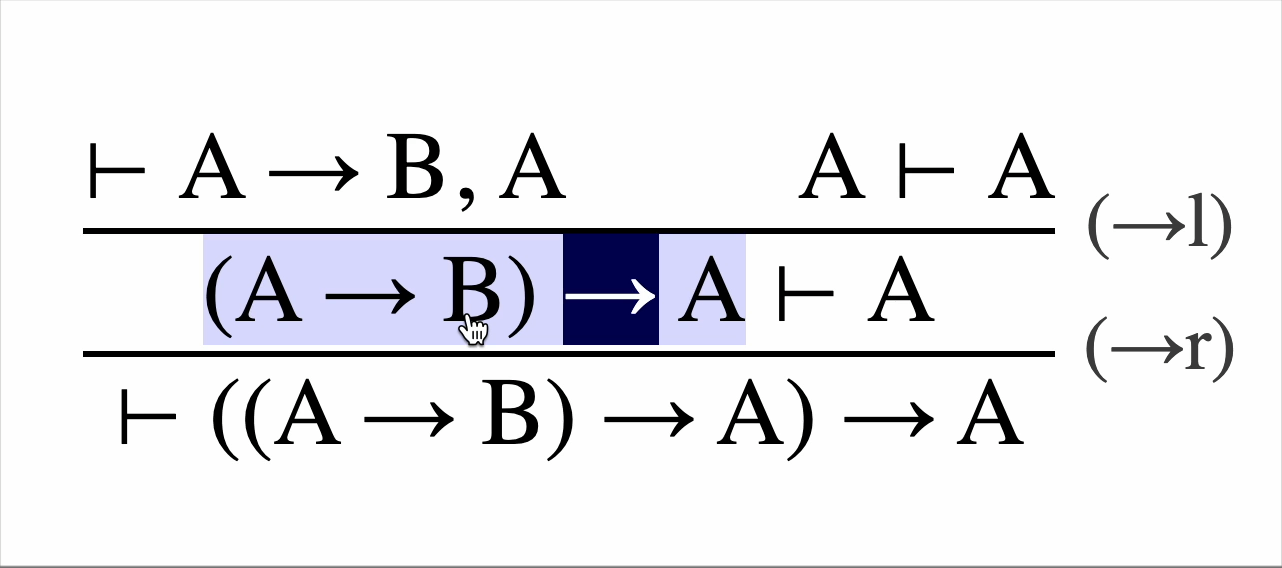
\includegraphics[width=\textwidth]{background/logitext-formula.png}
        \caption{Hovering over a formula}
    \end{subfigure}%
    \quad
    \begin{subfigure}{.48\textwidth}
        \centering
        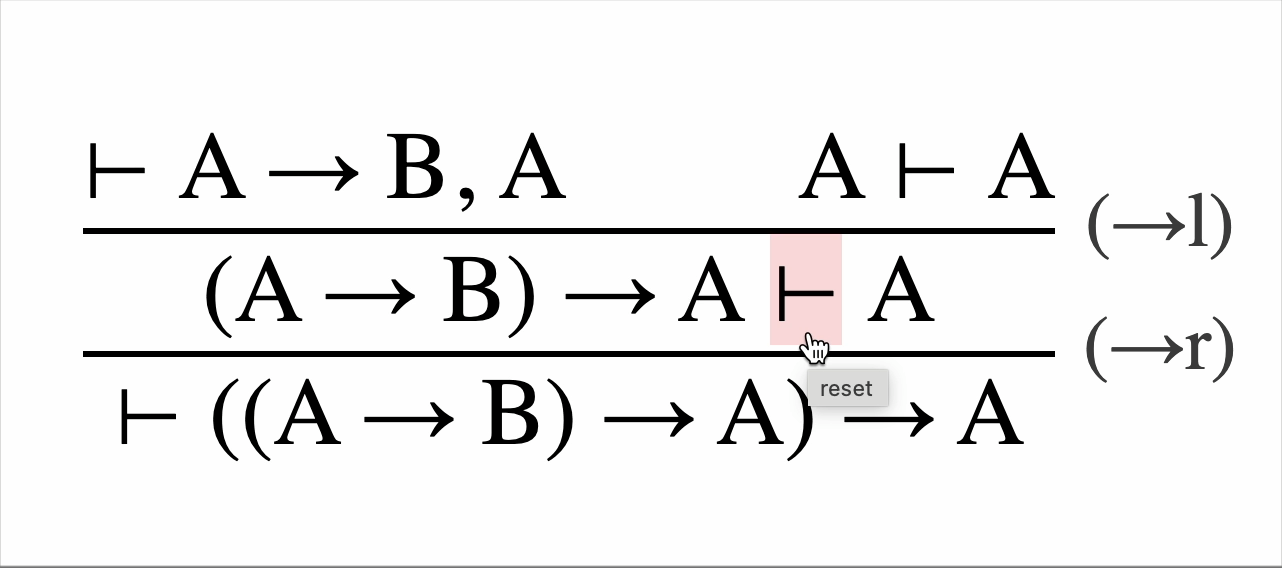
\includegraphics[width=\textwidth]{background/logitext-turnstile.png}
        \caption{Hovering over a turnstile}
    \end{subfigure}
    \caption{Lack of feedback when hovering over various parts of the derivation tree in Logitext}
    \label{fig:comparison:logitext}
\end{figure}

\paragraph{Helpful error messages}
When the user tries to apply an inference rule incorrectly, Logitext displays helpful and specific error messages, as seen in \Cref{fig:comparison:logitext-error}.

\begin{figure}[!htbp]
    \centering
    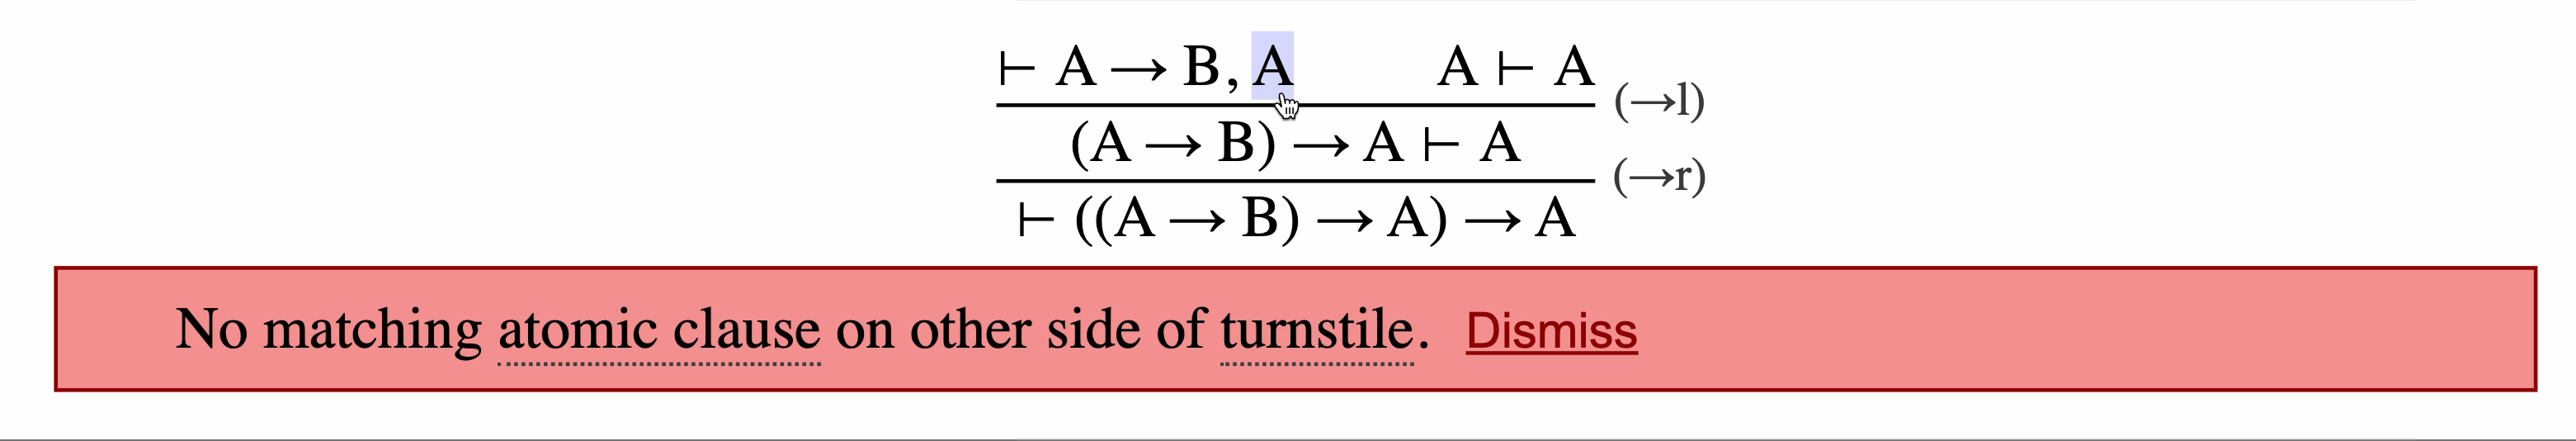
\includegraphics[width=\textwidth]{background/logitext-error.png}
    \caption{Helpful error messages in Logitext}
    \label{fig:comparison:logitext-error}
\end{figure}

\subsubsection{Flexibility}
Logitext only supports the system \textsc{lk}.

\subsection{Summary}
The application should retain the benefits and address the drawbacks of the proof assistants presented in this section. The desirable features of \projectname{} are as follows:
\begin{itemize}
    \item Users should be able to input statements in the application like writing statements by hand.
    \item The input syntax should either be already known by most users, or be easily accessible in the application.
    \item Users should be able to build derivations in the application like building derivations by hand.
    \item Users should be forced to think about which inference rule to apply and what the premises are. The application should not immediately rule out irrelevant inference rules.
    \item Users should be able to define both syntax and inference rules. The application should be as unopinionated about symbols as possible and designate as few special symbols as possible.
\end{itemize}
